\documentclass[11pt]{article}

\usepackage[letterpaper,margin=1in]{geometry}
\usepackage[T1]{fontenc}
\usepackage{lmodern}
\usepackage{microtype}
\usepackage{graphicx}
\usepackage{float}
\usepackage{booktabs}
\usepackage{tabularx}
\usepackage{enumitem}
\usepackage{xurl}
\usepackage{fancyvrb}
\usepackage{hyperref}

\hypersetup{hidelinks}
\setlist{itemsep=2pt,parsep=0pt,topsep=4pt,partopsep=0pt}
\graphicspath{{uml/rendered/}{screenshots/}}
\setlength{\parskip}{6pt plus 1pt minus 1pt}
\setlength{\parindent}{0pt}
\setlength{\emergencystretch}{5em}
\pagestyle{plain}
\urlstyle{same}

\newcommand{\field}[2]{\textbf{#1.} #2\par}
\newcommand{\shot}[2]{%
  \begin{figure}[H]
  \centering
  \includegraphics[width=\textwidth]{#1}
  \caption{#2}
  \end{figure}
}
\newcommand{\termshot}[2]{%
  \begin{figure}[H]
  \centering
  \includegraphics[width=\textwidth,height=0.82\textheight,keepaspectratio]{#1}
  \caption{#2}
  \end{figure}
}
\newcommand{\batchlines}[2]{%
  \VerbatimInput[fontsize=\footnotesize,firstline=#1,lastline=#2]{cli-batch-stdout.txt}
}

\begin{document}

\begin{titlepage}
\centering
\vspace*{0.75in}
{\Large York University\\[0.15em]}
{\large Lassonde School of Engineering\\[2.4em]}
{\Large EECS3311 -- Software Design\\[2.6em]}
{\Huge\bfseries Market Intelligence Agent\\[0.55em]}
{\Large Stage 2 -- Implementation Report\\[2.15in]}
\begin{tabular}{rl}
\textbf{Student:} & Erdem Calikoglu \\
\textbf{Student Number:} & 218188771 \\
\textbf{Instructor:} & Song Wang \\
\textbf{Date:} & November 8, 2026 \\
\textbf{Revised:} & November 22, 2026 \\
\end{tabular}
\vfill
\end{titlepage}

\tableofcontents
\newpage

\section{Project overview and implementation status}

I built a small research desk for one signed-in person. The Swing window and the terminal call the same Java services, and both read the same SQLite file, \texttt{data/market-intelligence.db}. You can ask for a quote, a company profile, ETF exposure, news, statements, a price history, or a sentiment score. You can also keep a portfolio and a watchlist. The desk does not place orders and it does not tell you to buy or sell.

Gemini is in two places, and only those two. If you ask why a price moved, the desk first loads the quote and the news, then asks Gemini to explain the move from what those articles say. If you type an ordinary sentence, Gemini may pick one allowed action, and it may write a short reply from the tool result. A plain quote never goes to the model. ``Say that more simply'' stays on the last reply and does not fetch anything new. Portfolio weights are calculated in Java. I do not send those numbers to Gemini.

The model I ship with is \texttt{gemini-3.5-flash-lite}. Flash-Lite uses minimal thinking, because a longer thinking pass was eating the token budget and the note stopped after the price. If \texttt{GEMINI\_MODEL} is set to \texttt{gemini-3.8-flash} or \texttt{gemini-2.5-flash}, unset it. The first one thought too long. The second one returned HTTP 404 on a new key.

The box at the bottom of the window is a message field. Enter sends, Shift+Enter adds a line, and the reply stays in the conversation. The terminal takes the same words. A leading slash still works, but you do not need it.

What works today, when the matching key is set:

\begin{itemize}
\item Register, sign in, and sign out. The create-account screen and the sign-on screen are separate.
\item Quotes, overviews, comparison, news, ETF sector weights, overlap, portfolio edits, and a watchlist.
\item Country exposure. Finnhub's published report if the plan allows it. Otherwise the headquarters country of at most 25 holdings.
\item Portfolio exposure as price times quantity, with currencies kept apart.
\item A move note that uses the articles, then the quote and the sources underneath.
\item Statements, daily bars with RSI, and one sentiment score.
\item A home screen with portfolio value, the day move, one row per position, and a sliding tape.
\item A non-interactive command line. \texttt{java -jar target/Agent.jar -LLMAPI -input task.txt} runs \texttt{task.txt} and exits. Section~\ref{sec:batch-cli}.
\end{itemize}

What I am not going to dress up:

\begin{itemize}
\item The demonstration is one public recording. The timestamps are in Section~\ref{sec:demos}.
\item On the free Finnhub plan, country weights are headquarters of the holdings I could look up. They are not the fund's factsheet and they are not revenue. Anything unknown stays unknown.
\item Finnhub's free quotes are US listings. \texttt{XEQT.TO} stays unpriced, and the screen says so.
\item Alpha Vantage company overview is a paid endpoint. I use Alpha Vantage for ETF holdings.
\item If a live call fails, the router does not try the next vendor.
\item The model cannot add or remove a position.
\item A sentence that tries to override the instructions does not run a tool.
\end{itemize}

\section{Feature to implementation mapping}
\label{sec:features}

Stage~1 had UC-01 through UC-16. I kept all of them. UC-17, UC-18, and UC-19 are the statement, history, and sentiment commands I added once those free APIs were wired in. UC-20 is the home screen. The batch command line in Section~\ref{sec:batch-cli} is the Stage~2 update that Stage~3 will call.

Each feature below states the original requirement, how this desk implements it, and where the running code differs. Where I could run the command with no provider key, the listing is standard output from this command, captured on 20~November 2026:

\begin{quote}
\texttt{java -jar target/Agent.jar -LLMAPI -input task.txt}
\end{quote}

The process used a fresh SQLite file and no API keys. The terminal draws boxes and a bullet between quantity and type. This PDF replaces those characters so pdfLaTeX can embed the same text. The unmodified capture is \texttt{docs/stage2/cli-batch-transcript.txt}. Standard error from that run is included with the batch-CLI feature.

The window figures were taken on this branch, signed in as \texttt{erdem.demo}, with the provider keys set. Passwords are masked. The terminal figures in Section~\ref{sec:batch-cli} are the same jar with those keys. Section~\ref{sec:shots} indexes the files.

\subsection{UC-01 Register account}
\label{uc01}

\paragraph{Original requirement.}
Stage~1 UC-01. The user chooses registration. The system asks for a username and a password, validates both, rejects a name that is already registered or input that fails the rules, hashes the password, stores the hash with the new user, and confirms success. If saving fails, the account is not created. Afterward a new account exists.

\paragraph{Implementation.}
The create-account screen is separate from sign-on. \texttt{AuthenticationPanel} collects the form and asks for the password twice. \texttt{SessionWorkspace.register} calls \texttt{AuthService.register}. The username must be 3 to 30 characters from \texttt{A-Z}, \texttt{a-z}, digits, and \texttt{.\_-}. The password must be at least 8 characters. \texttt{BCryptPasswordHasher} hashes it. \texttt{SQLiteUserRepository.save} stores the row. The window then returns to sign-on. The new user is not logged in yet. A taken name or a short password is rejected, and the password is not written to the status line. This path does not call Gemini.

Batch mode uses the same \texttt{AuthService}. \texttt{BatchSession} creates the local demo account when it is missing, and \texttt{--register} creates the account named by \texttt{--user}. The confirmation line is \texttt{Created local account \ldots}.

\paragraph{Deviation.}
Stage~1 described one registration flow and did not describe a second interface. The window still matches that flow: confirm, then go back to sign-on, still signed out. The batch path creates the account and signs in immediately, because a task file has to run without a second prompt. The password is the local demo password or the one passed to \texttt{--register}. It is not printed. A name that already exists is still rejected, and a wrong password on a later sign-in does not reveal which field failed.

\paragraph{Evidence.}
\batchlines{1}{1}

\shot{uc01-a.png}{Create-account form for erdem.demo. The password and the confirmation are masked.}
\shot{uc01-b.png}{Back on sign-on. The status says the account erdem.demo was created.}

\subsection{UC-02 Log in}
\label{uc02}

\paragraph{Original requirement.}
Stage~1 UC-02. The user submits a username and a password. \texttt{AuthService} loads the user and checks the hash. \texttt{SessionManager} starts a session. The user's portfolio, watchlist, preferences, and memory become available, and the terminal shows the authenticated home screen. A failed sign-in does not say whether the name or the password was wrong.

\paragraph{Implementation.}
Sign-on does not ask the user to type the password twice. \texttt{AuthenticationPanel} and \texttt{TerminalUI.login} call \texttt{AuthService.authenticate} and \texttt{PasswordHasher.verify}, then \texttt{SessionManager.startSession}. A wrong password stays on that screen with \texttt{Invalid username or password.} Batch mode does not prompt. \texttt{BatchSession.signIn} opens the session, and the next line of output names the account. \texttt{whoami} prints the user id and the login time from \texttt{UserSession}.

\paragraph{Deviation.}
There is no \texttt{UserPreferences} class. Conversation rows are stored per user and are read on a follow-up, not dumped at login. The interactive menu is unchanged when the jar is started with no batch flag. Batch mode skips the menu. With no \texttt{--user} and no \texttt{MI\_USERNAME}, it signs in as the local demo account \texttt{guest} so \texttt{-input task.txt} runs without typing. \texttt{--user} and \texttt{--password}, or \texttt{MI\_USERNAME} and \texttt{MI\_PASSWORD}, select another account. \texttt{--guest} and \texttt{MI\_GUEST=1} force the demo account.

\paragraph{Evidence.}
\batchlines{2}{12}

\shot{uc02-a.png}{Rejected sign-on. The message does not say whether the name or the password was wrong.}
\shot{uc02-b.png}{Signed-in home for erdem.demo. The tape is loaded and the portfolio is empty.}

\subsection{UC-03 Log out}
\label{uc03}

\paragraph{Original requirement.}
Stage~1 UC-03. An authenticated user requests logout. Required user state is persisted, the session is invalidated, in-memory session state is cleared, and the application returns to the login screen. Afterward no session is active.

\paragraph{Implementation.}
\texttt{TerminalUI.logout} and \texttt{SessionWorkspace.logout} call \texttt{endSession} on \texttt{SessionManager}. The portfolio and watchlist rows stay in SQLite under that user. The next interactive command asks for sign-in again. In batch mode the logout line is printed and \texttt{runBatch} stops, so later lines in the file are not run.

\paragraph{Deviation.}
Portfolio and watchlist writes are persisted when the command runs, not again at logout. There is no separate session row to flush. The interactive terminal still returns to the auth menu, and the window still returns to sign-on. Batch mode exits instead of drawing that menu, because waiting for a key would block a non-interactive run.

\paragraph{Evidence.}
\batchlines{69}{73}

\shot{uc03-a.png}{Sign-on after logout. The status is signed out.}

\subsection{UC-04 Get a market quote}
\label{uc04}

\paragraph{Original requirement.}
Stage~1 UC-04. An authenticated user requests a quote by a command or by natural language. The symbol is validated, the market-data tool is selected, the provider is queried, a \texttt{MarketQuote} is built, and the price is displayed. An invalid symbol is rejected before the call. If the provider is unavailable, the failure is explicit.

\paragraph{Implementation.}
\texttt{quote NVDA}, or \texttt{QUOTE NVDA} in the window, is parsed by \texttt{CommandParser} or \texttt{DeskCommand}. \texttt{TerminalUI} builds a \texttt{ToolRequest} for \texttt{ActionType.MARKET\_QUOTE}. \texttt{MarketDataTool} checks the symbol and calls \texttt{ProviderRouter.getQuote}. Finnhub is registered first when \texttt{FINNHUB\_API\_KEY} is set. Twelve Data, then Alpha Vantage, are used only when an earlier adapter was never registered. A failed call does not hop to the next vendor. The screen shows price, previous close, and percent change. The symbol is remembered so a later ``it'' can use it. Gemini is not called. Batch mode runs this same handler and prints the result without clearing the screen.

\paragraph{Deviation.}
Stage~1 sent the research use cases through the model. A direct quote no longer does. The router is not a failover chain. On the free Finnhub plan a non-US symbol such as \texttt{XEQT.TO} stays unpriced and the screen says so. With no quote key, the tool is not registered and the command reports that, which is what the standard-error listing in Section~\ref{sec:batch-cli} shows. That line is the offline failure. The window figure below is the live quote.

\paragraph{Evidence.}
\shot{uc04-a.png}{QUOTE NVDA. Price 125.53, previous close 145.90, change $-14.0088\%$.}

\subsection{UC-05 Get a security overview}
\label{uc05}

\paragraph{Original requirement.}
Stage~1 UC-05. The user asks for an overview. The symbol is validated, \texttt{MarketDataTool} requests security metadata, the provider result is mapped to a \texttt{SecurityOverview}, and the response is displayed.

\paragraph{Implementation.}
\texttt{overview NVDA} follows the quote path and calls \texttt{getSecurityOverview} on \texttt{ProviderRouter}. Finnhub's free profile supplies the name, exchange, currency, and an industry label. The screen says when the profile has no company description. An ETF often has no profile. The same command works in batch mode. Gemini is not called.

\paragraph{Deviation.}
Same as the quote: the model is not on this command. Alpha Vantage company overview is a premium endpoint, so it is not the source I rely on. If neither Finnhub nor Alpha Vantage is configured, the command says the overview is unavailable.

\paragraph{Evidence.}
\shot{uc05-a.png}{OVERVIEW NVDA. NVIDIA Corporation, NASDAQ NMS, USD, Semiconductors, and the Finnhub headquarters note.}

\subsection{UC-06 Analyze ETF exposure}
\label{uc06}

\paragraph{Original requirement.}
Stage~1 UC-06. The user asks for the sector or geographic composition of an ETF. The symbol is validated, \texttt{ETFExposureTool} retrieves holdings, \texttt{ExposureCalculator} produces an \texttt{ExposureResult}, and the LLM explains that result. If the holdings are not sufficient, the system says the exposure cannot be calculated.

\paragraph{Implementation.}
\texttt{sector QQQ} loads the ETF profile and reports the provider's sector weights. \texttt{geography QQQ} and \texttt{geo QQQ} try Finnhub's published country report. On HTTP 403, \texttt{HoldingCountryResolver} maps at most 25 holdings to headquarters countries from Finnhub profiles. A holding with no profile stays Unknown. Weight the provider left blank stays unassigned and is named in the note. \texttt{geography NVDA} has nothing to break down, because a stock has no holdings list. \texttt{ProviderText.redact} strips a key if a vendor echoes one. Gemini is not asked to narrate the weights.

\paragraph{Deviation.}
Stage~1 ended this use case with an LLM explanation. I show the weights and stop. Country weights on the free plan are headquarters of the holdings I could look up. They are not the fund's factsheet and they are not revenue. Sector weights come from the provider's sector breakdown on the profile, not from a second invented allocation. Both \texttt{ALPHA\_VANTAGE\_API\_KEY} and \texttt{FINNHUB\_API\_KEY} are required for the headquarters fallback.

\paragraph{Evidence.}
\shot{uc06-a.png}{SECTOR QQQ. Information technology leads at 52.70\%, then the remaining sectors.}
\shot{uc06-b.png}{GEOGRAPHY QQQ. Headquarters weights, led by the United States, with the note that these are not the factsheet.}
\shot{uc06-c.png}{GEOGRAPHY NVDA. A stock has no holdings list, so no country breakdown is estimated.}

\subsection{UC-07 Compare securities}
\label{uc07}

\paragraph{Original requirement.}
Stage~1 UC-07. The user names two symbols. The planner decides what to fetch, the tools run, \texttt{ComparisonTool} builds the comparison, and the composer presents it. If one symbol cannot be retrieved, the other is not silently substituted.

\paragraph{Implementation.}
\texttt{compare NVDA MSFT} loads two quotes through \texttt{ComparisonTool} and \texttt{ProviderRouter}. \texttt{SecurityComparisonCalculator} subtracts the percent changes. The screen shows each price, each previous close, each percent change, and the gap in percentage points. One symbol is not enough, and the desk asks for the second. Gemini is not called.

\paragraph{Deviation.}
The direct command does not go through \texttt{RequestPlanner} or the model. Stage~1 had the planner choose the tools. Here the verb selects \texttt{ActionType.SECURITY\_COMPARISON} itself. A follow-up sentence can still reach the same tool through UC-16, and that path still requires two symbols.

\paragraph{Evidence.}
\shot{uc07-a.png}{COMPARE NVDA MSFT. NVDA $-14.0088\%$, MSFT $-2.7954\%$, gap $-11.2134\%$.}

\subsection{UC-08 Analyze ETF overlap}
\label{uc08}

\paragraph{Original requirement.}
Stage~1 UC-08. The user names two ETFs. Holdings are loaded for each, \texttt{ExposureCalculator} finds the common names and the overlap percentage, an \texttt{OverlapResult} is produced, and the result is explained and displayed. If either holding list is missing, the overlap is not calculated.

\paragraph{Implementation.}
\texttt{overlap QQQ SPY} loads both lists through \texttt{AlphaVantageAdapter} and the router. \texttt{ExposureCalculator.calculateOverlap} reports the shared weight and up to 15 common holdings. Gemini is not called.

\paragraph{Deviation.}
Stage~1 said the result is explained. I display the overlap and the shared names, and I do not send them to the model. The holding source is Alpha Vantage, because Finnhub's fund datasets are not on the free plan this desk uses.

\paragraph{Evidence.}
\shot{uc08-a.png}{OVERLAP QQQ SPY, top of the result. Overlap 52.03\%, shared holdings starting with AAPL.}
\shot{uc08-b.png}{The same overlap, scrolled to the end of the shared-holdings list.}

\subsection{UC-09 Retrieve financial news}
\label{uc09}

\paragraph{Original requirement.}
Stage~1 UC-09. The user asks for recent news. \texttt{NewsTool} validates the symbol, \texttt{NewsProvider} returns articles, they are mapped to \texttt{NewsArticle}, the LLM summarizes them, and the article metadata is included. If nothing qualifies, the system says so.

\paragraph{Implementation.}
\texttt{news NVDA} calls \texttt{NewsTool} and \texttt{ProviderRouter.getNews}. Marketaux is used when \texttt{MARKETAUX\_API\_TOKEN} is set. Otherwise Finnhub company news is used. Alpha Vantage news is not registered, because that free plan is about 25 calls a day. The list shows title, source, time, URL, and Marketaux sentiment when the article has it. A headline match means the ticker was attached to the article. It does not, by itself, mean the article caused a move. Asking why the price moved is UC-10.

\paragraph{Deviation.}
The news command does not ask Gemini to summarize the list. Stage~1 put a summary on this use case. A spoken reply on top of the articles, when the user types a sentence and Gemini is configured, is UC-16 and has to stick to the article text. With no news key the command says news is unavailable.

\paragraph{Evidence.}
\shot{uc09-a.png}{NEWS NVDA. Three headlines with source, published time, URL, and provider sentiment.}

\subsection{UC-10 Explain a recent move}
\label{uc10}

\paragraph{Original requirement.}
Stage~1 UC-10. The user asks why a price moved. The planner fetches a quote and recent news, both results are validated, and the LLM writes an explanation constrained to that data. If one source fails, the reply says what is missing. The system must not invent a cause when the supporting information was not retrieved.

\paragraph{Implementation.}
\texttt{why NVDA} and a sentence such as \texttt{why did microsoft fall} both land on this path. \texttt{why MSFT} is the symbol form. A longer sentence is a follow-up, not a ticker. \texttt{MarketMovementTool} loads the quote and up to three articles. \texttt{NewsTiming} marks anything published after the last trade. \texttt{MarketExplanationService.explain} calls \texttt{GeminiLLMClient.generate}, not the short call, and Flash-Lite is told to think as little as possible so the note is not cut off after the price. The note names the symbol, the price, and the percent change, then explains the move from what the articles say and attributes each reason to the reporting. An article after the last trade is later context, not proof it caused that print. If no article states a reason, the note says the evidence does not establish a cause. It does not recommend a buy or a sell. The answer is shown first. The quote and the sources follow. \texttt{nasdaq} is read as \texttt{QQQ}, and the note has to say QQQ is an ETF.

\paragraph{Deviation.}
Stage~1 had the composer ask the model even when evidence was missing. I load the quote and the news first, and I do not show a note that was cut off by the token limit. The shipped model is \texttt{gemini-3.5-flash-lite}. If \texttt{GEMINI\_MODEL} is set to \texttt{gemini-3.8-flash} or \texttt{gemini-2.5-flash}, unset it. The \texttt{-LLMAPI} flag records that this run expects the model. It does not carry the key. With no \texttt{GEMINI\_API\_KEY} the quote and the news still show, and the desk says the explanation is unavailable. The batch listing in Section~\ref{sec:batch-cli} had no key. The window figure below is a finished note from a run that had one.

\paragraph{Evidence.}
\shot{uc10-a.png}{WHY NVDA. The note cites the articles. The quote and the numbered source URLs follow.}

\subsection{UC-11 Add a portfolio position}
\label{uc11}

\paragraph{Original requirement.}
Stage~1 UC-11. The user asks to add a position. The symbol and quantity are validated, a \texttt{PortfolioPosition} is created, \texttt{PortfolioService} loads that user's portfolio, the position is added, \texttt{PortfolioRepository} persists it, and the system confirms the change. The position belongs to the authenticated user.

\paragraph{Implementation.}
\texttt{portfolio add NVDA 10 STOCK}, and \texttt{PORT ADD NVDA 10 STOCK} in the window, call \texttt{SessionWorkspace.addPosition}, then \texttt{PortfolioService}, then \texttt{SQLitePortfolioRepository}. The type is \texttt{STOCK}, \texttt{ETF}, or \texttt{OTHER}. The confirmation is the line \texttt{NVDA added to portfolio.} A sentence cannot add a position. The planner allowlist does not include this action.

\paragraph{Deviation.}
Stage~1 put add on the agent tools. I moved it off the model so a sentence cannot change what I hold. The terminal form also requires the asset type, which Stage~1's step list did not name. Batch mode runs the same command and prints the confirmation without a prompt.

\paragraph{Evidence.}
\batchlines{20}{35}

\shot{uc11-a.png}{Portfolio screen after PORT ADD NVDA 10 STOCK. The row is saved.}

\subsection{UC-12 Remove a portfolio position}
\label{uc12}

\paragraph{Original requirement.}
Stage~1 UC-12. The user names a symbol. The portfolio is loaded, the matching position is removed, the update is persisted, and the system confirms it. If the position is not there, the portfolio is unchanged and the user is told.

\paragraph{Implementation.}
\texttt{portfolio remove NVDA} and \texttt{PORT REMOVE NVDA} call \texttt{removePosition} on \texttt{PortfolioService}. A missing symbol prints that it is not in the portfolio and leaves the other rows. The model cannot do this.

\paragraph{Deviation.}
Same reason as add: removal is not an agent tool. Batch mode stops the file after \texttt{logout}, so a remove has to appear before that line. The capture below removes NVDA, which was held, and the next listing shows only QQQ.

\paragraph{Evidence.}
\batchlines{47}{57}

\shot{uc12-a.png}{After PORT REMOVE MSFT. NVDA remains, and the status says the position was removed.}
\shot{uc12-b.png}{After PORT REMOVE TSLA, which is not held. NVDA remains.}

\subsection{UC-13 View the portfolio}
\label{uc13}

\paragraph{Original requirement.}
Stage~1 UC-13. \texttt{SessionManager} identifies the user, \texttt{PortfolioService} loads that portfolio, the positions are formatted, and the portfolio is displayed. The stored rows do not change.

\paragraph{Implementation.}
\texttt{portfolio} with no arguments, or the Portfolio screen, lists the stored symbol, quantity, and type. No network call is required just to list the rows. Prices show up on the home screen and on \texttt{portfolio exposure} when a quote is available. Batch mode prints the same table.

\paragraph{Deviation.}
Stage~1 described the terminal list. The window shows the same rows and, when quotes exist, the market value. Listing the rows still does not require a provider. An empty portfolio says \texttt{No positions}, which is the first portfolio block in the capture.

\paragraph{Evidence.}
\batchlines{14}{18}
\batchlines{28}{35}

\shot{uc13-a.png}{Portfolio screen listing the stored NVDA position.}

\subsection{UC-14 Manage the watchlist}
\label{uc14}

\paragraph{Original requirement.}
Stage~1 UC-14. The user adds, removes, or views watchlist symbols. The symbol is validated when one is required, \texttt{WatchlistService} loads that user's list, the change is persisted when there is one, and the current list is displayed.

\paragraph{Implementation.}
\texttt{watchlist}, \texttt{watchlist add AAPL}, and \texttt{watchlist remove AAPL} go through \texttt{WatchlistService} and \texttt{SQLiteWatchlistRepository}. The window accepts \texttt{WATCH ADD} and \texttt{WATCH REMOVE}. A watchlist item has no quantity. A missing symbol on remove is reported and the other symbols stay.

\paragraph{Deviation.}
There is no \texttt{WatchlistTool} on the agent. A sentence cannot add or remove a symbol. Stage~1 did not require a quantity, and the implementation does not add one.

\paragraph{Evidence.}
\batchlines{37}{45}
\batchlines{59}{67}

\shot{uc14-a.png}{Watchlist with AAPL added.}
\shot{uc14-b.png}{Watchlist after AAPL was removed. The monitor is empty.}

\subsection{UC-15 Analyze portfolio exposure}
\label{uc15}

\paragraph{Original requirement.}
Stage~1 UC-15. The user's portfolio is loaded, stock and ETF positions are identified, ETF holdings are retrieved where required, quantities and weights are combined, \texttt{ExposureCalculator} produces an aggregate result, and the LLM explains it. If an ETF cannot be retrieved, the missing position is named and the analysis is not presented as complete.

\paragraph{Implementation.}
\texttt{portfolio exposure} and \texttt{EXPOSURE} call \texttt{PortfolioAnalysisTool} and \texttt{PortfolioExposureCalculator}. Value is price times quantity. Day move is the price change times quantity. Currencies stay in separate books. A position with no price is named and left out of the total. ETF sector weights are look-through when the holding list exists. If a sentence selects this action, the numbers still are not sent to the model. \texttt{PortfolioBook} is the home-screen summary of the same figures.

\paragraph{Deviation.}
Stage~1 had the model explain the exposure. The figure is arithmetic, and narrating it invited a recommendation, so Gemini does not see these numbers. The batch listing had no quote key. The window figures below are the priced exposure from a run that had one.

\paragraph{Evidence.}
\shot{uc15-a.png}{Portfolio with NVDA 10 STOCK and QQQ 3 ETF before the exposure report.}
\shot{uc15-b.png}{EXPOSURE, top. USD book value 3,080.65 and the sector weights.}
\shot{uc15-c.png}{EXPOSURE, bottom. Look-through holdings of QQQ and the currency note.}

\subsection{UC-16 Ask a follow-up}
\label{uc16}

\paragraph{Original requirement.}
Stage~1 UC-16. The user continues a conversation without repeating the entity. Recent context is loaded, the previous entity is identified, \texttt{RequestPlanner} builds a plan, the tools run, a response is generated, and both sides are stored. If the reference is ambiguous, the system asks instead of guessing.

\paragraph{Implementation.}
The window's message box and a non-verb line in the terminal both call \texttt{ResearchGateway.ask} and \texttt{AgentController.handle}. \texttt{ConversationMemory} reads recent turns and the last symbol for that user. \texttt{RequestPlanner} always builds a keyword plan first. If Gemini is configured, it may replace that plan with one allowed JSON action. A bad reply falls back to the keywords. A lookup runs through \texttt{ToolManager}. A move plan then uses UC-10. ``Say that more simply'' is \texttt{DISCUSS}: nothing is fetched, and Gemini rewrites the stored exchange. Portfolio figures are left out of that prompt. Another user's rows are never read. A sentence that says to ignore previous instructions, or that looks like SQL, is rejected and does not run a tool. Compare and overlap still need two symbols. Home and tape refreshes do not replace the remembered symbol.

\paragraph{Deviation.}
The class is \texttt{ConversationMemory}, not a type named \texttt{MemoryService}. The model may only name an allowed action. Add, remove, and watchlist edits are not on that list. A rephrase does not run a tool. Stage~1 had the model more free to choose the next step. Keyword planning still works when \texttt{GEMINI\_API\_KEY} is unset. The window figures below are the live exchange: the sector question, a shorter wording, and a sentence that tries to override the instructions.

\paragraph{Evidence.}
\shot{uc16-a.png}{Chat follow-up asking for the sector exposure of the last symbol. NVDA has no ETF weights.}
\shot{uc16-b.png}{The same chat after ``say that more simply.'' The reply is shorter, and no new quote was fetched.}
\shot{uc16-c.png}{A sentence that tells the desk to ignore its instructions. No tool ran.}

\subsection{UC-17 Read financial statements}
\label{uc17}

\paragraph{Original requirement.}
This was not a Stage~1 use case. I added it so the Financial Modeling Prep adapter is something a person can run, not only a class behind the router.

\paragraph{Implementation.}
\texttt{statements NVDA} goes through \texttt{MarketInsightTool}.\\
The adapter is \texttt{FinancialModelingPrepAdapter}.
The method is \texttt{getFinancialStatements}. I show up to four annual periods of the income statement, the balance sheet, and the cash-flow statement. A line the filing omitted stays blank. Without \texttt{FMP\_API\_KEY} the command says it is unavailable. Gemini is not called.

\paragraph{Deviation.}
There was no Stage~1 requirement to depart from. The command does not replace a Stage~1 feature. It uses three provider calls on a plan of about 250 requests a day.

\paragraph{Evidence.}
\shot{uc17-a.png}{STATEMENTS NVDA, top. Annual figures from Financial Modeling Prep, including the latest two years.}
\shot{uc17-b.png}{STATEMENTS NVDA, lower years. Income, balance sheet, and cash flow for the earlier filings.}

\subsection{UC-18 Read price history}
\label{uc18}

\paragraph{Original requirement.}
This was not a Stage~1 use case. I added it so the Twelve Data adapter is visible as a command.

\paragraph{Implementation.}
\texttt{history NVDA} asks Twelve Data for recent daily bars and the latest 14-day RSI through \texttt{MarketInsightTool} and \texttt{TwelveDataAdapter}. The screen shows the eight newest bars. Quotes still work from Finnhub if this key is missing. Gemini is not called.

\paragraph{Deviation.}
There was no Stage~1 requirement to depart from. \texttt{history} is unavailable when \texttt{TWELVE\_DATA\_API\_KEY} is unset, and that does not remove quotes.

\paragraph{Evidence.}
\shot{uc18-a.png}{HISTORY NVDA. Eight daily bars and a 14-day RSI of 15.05 from Twelve Data.}

\subsection{UC-19 Read sentiment}
\label{uc19}

\paragraph{Original requirement.}
This was not a Stage~1 use case. I added it so the SentiSense adapter is visible as a command.

\paragraph{Implementation.}
\texttt{sentiment NVDA} asks SentiSense for the latest score, from $-1$ to $1$, through \texttt{MarketInsightTool} and \texttt{SentiSenseAdapter}. \texttt{SentimentBands} supplies the label for that score. The band is a label, not advice. Article sentiment from Marketaux is a different field and stays on the article. Gemini is not called.

\paragraph{Deviation.}
There was no Stage~1 requirement to depart from. I did not buy a paid SentiSense plan. Without \texttt{SENTISENSE\_API\_KEY} the command says it is unavailable.

\paragraph{Evidence.}
\shot{uc19-a.png}{SENTIMENT NVDA. Score about $-0.107$, labeled Neutral, from SentiSense.}

\subsection{UC-20 View the home desk}
\label{uc20}

\paragraph{Original requirement.}
This was not a Stage~1 use case. Stage~1 was a terminal. I added the home screen so the window can show the book and a tape after sign-on.

\paragraph{Implementation.}
After sign-on, F1 shows market value, the day move, one row per position sorted by market value, a stacked allocation bar, and a tape of index quotes, portfolio quotes, and a few headlines. \texttt{DashboardPanel} asks \texttt{PortfolioBook} for the figures and \texttt{TapeLine} for the tape. Network calls run off the Swing thread through \texttt{BackgroundWork}. Unpriced positions stay named and are left out of the total. Holdings refresh on the same 90-second cadence as the tape. A later refresh keeps the last totals until the new quotes return. The terminal has no tape. The same positions are listed by \texttt{portfolio}.

\paragraph{Deviation.}
Stage~1 had no window, so this screen is new rather than a change to a specified flow. The terminal batch run has no tape. The home figure below is the window.

\paragraph{Evidence.}
\shot{uc20-a.png}{Home desk. Market value 3,080.65, day move $-314.27$ ($-9.26\%$), QQQ and NVDA rows, and the headline tape.}

\section{Non-interactive command line}
\label{sec:batch-cli}

\paragraph{Original requirement.}
The Stage~2 update says: provide a version of the agent that users can run directly from a terminal. For example, \texttt{java -jar Agent.jar -LLMAPI -input task.txt} should run the agent on the task specified in \texttt{task.txt}. Document the supported options and provide a working example in the README. The CLI must accept input from a file, standard input, an API call, or another supported method. The CLI is required for Stage~3.

\paragraph{Implementation.}
\texttt{./mvnw -DskipTests package} builds \texttt{target/Agent.jar}. The Maven Shade plugin puts the dependencies in that jar and sets \texttt{Main-Class} to \texttt{com.marketintel.Main}. \texttt{CliOptions} accepts \texttt{-input}, \texttt{-c} or \texttt{--command}, \texttt{--batch}, \texttt{-LLMAPI}, \texttt{--guest}, \texttt{--user}, \texttt{--password}, \texttt{--register}, \texttt{--database}, \texttt{--cli}, and \texttt{--gui}. \texttt{StdinProbe} treats a pipe as batch input and leaves \texttt{./mvnw exec:java} interactive, because that launch often has no Java console. \texttt{BatchRunner} reads the lines, \texttt{BatchSession} signs in, and \texttt{TerminalUI.runBatch} runs the same verbs as the interactive terminal. Blank lines and lines that start with \texttt{\#} are skipped. Results go to standard output. The process then exits. \texttt{logout} and \texttt{exit} stop the file. A command that fails sets status 1 and the rest of the file still runs. Status 2 means the arguments, the file, or the sign-in could not be used.

The interactive menu and the Swing window are the same paths as before when no batch flag is present and standard input is a terminal.

\paragraph{Deviation.}
The jar is \texttt{target/Agent.jar}, not a file named \texttt{Agent.jar} dropped in the working directory. The command to build it, and the working example, are in the README. \texttt{-LLMAPI} does not take a key on the command line. A key in the process list would be a secret, so the Gemini key stays in \texttt{GEMINI\_API\_KEY}. If the flag is set and the key is missing, the run says so and continues. There is no HTTP endpoint on this desk, so ``an API call'' is not a fourth transport. The supported inputs are a file, standard input, and one inline command. Batch mode cannot stop at the login menu. When no account is given, it signs in as the local demo user \texttt{guest} with password \texttt{guest-demo}, creating that row in SQLite if needed. That password is a local demo password, not an API key. \texttt{--user} or \texttt{MI\_USERNAME} overrides it.

\paragraph{Evidence.}
The listing is the offline run named above, from a fresh database with no provider keys. Standard error is the provider warnings from that process. No key value is in either listing. The figures after it are \texttt{target/Agent.jar} on this branch with the keys set. The password is not on screen.

\VerbatimInput[fontsize=\footnotesize]{cli-batch-stdout.txt}

\VerbatimInput[fontsize=\footnotesize]{cli-batch-stderr.txt}

\termshot{cli-01-batch.png}{\texttt{java -jar target/Agent.jar -LLMAPI -input task.txt}. The demo account runs the task file and exits.}
\termshot{cli-02-quote.png}{\texttt{-c "quote NVDA"}. Live price 125.53, previous close 145.98, change $-14.0088\%$.}
\termshot{cli-03-news.png}{\texttt{-c "news NVDA"}. Three headlines with source, time, sentiment, and URL.}
\termshot{cli-04-why.png}{\texttt{-c "why NVDA"}. The Gemini note, the quote, and the numbered sources.}
\termshot{cli-05-stdin.png}{A pipe into \texttt{-input -}. \texttt{quote MSFT} prints the live quote and the process exits.}
\termshot{cli-06-interactive.png}{Interactive REPL. Guest signs in and \texttt{quote NVDA} prints the live price.}

\section{Screenshot index}
\label{sec:shots}

The window shots sit beside each feature in Section~\ref{sec:features}. The terminal shots sit in Section~\ref{sec:batch-cli}. They were taken on this branch with the provider keys set. The window session is \texttt{erdem.demo}. The terminal session is the local demo user \texttt{guest}. Password fields are masked, and no key is on screen. The files are in \texttt{docs/stage2/screenshots/}.

\begin{itemize}
\item UC-01. \texttt{uc01-a.png} create-account form. \texttt{uc01-b.png} return to sign-on.
\item UC-02. \texttt{uc02-a.png} rejected sign-on. \texttt{uc02-b.png} signed-in home.
\item UC-03. \texttt{uc03-a.png} sign-on after logout.
\item UC-04. \texttt{uc04-a.png} \texttt{QUOTE NVDA}.
\item UC-05. \texttt{uc05-a.png} \texttt{OVERVIEW NVDA}.
\item UC-06. \texttt{uc06-a.png} \texttt{SECTOR QQQ}. \texttt{uc06-b.png} \texttt{GEOGRAPHY QQQ}. \texttt{uc06-c.png} \texttt{GEOGRAPHY NVDA}.
\item UC-07. \texttt{uc07-a.png} \texttt{COMPARE NVDA MSFT}.
\item UC-08. \texttt{uc08-a.png} and \texttt{uc08-b.png}. \texttt{OVERLAP QQQ SPY}, top and bottom of the list.
\item UC-09. \texttt{uc09-a.png} \texttt{NEWS NVDA}.
\item UC-10. \texttt{uc10-a.png} \texttt{WHY NVDA}.
\item UC-11. \texttt{uc11-a.png} portfolio after \texttt{PORT ADD NVDA 10 STOCK}.
\item UC-12. \texttt{uc12-a.png} a held symbol removed. \texttt{uc12-b.png} a missing symbol.
\item UC-13. \texttt{uc13-a.png} the stored portfolio.
\item UC-14. \texttt{uc14-a.png} watchlist with AAPL. \texttt{uc14-b.png} the empty watchlist.
\item UC-15. \texttt{uc15-a.png} the two positions. \texttt{uc15-b.png} and \texttt{uc15-c.png} the priced exposure.
\item UC-16. \texttt{uc16-a.png} the sector follow-up. \texttt{uc16-b.png} a shorter wording. \texttt{uc16-c.png} a rejected instruction.
\item UC-17. \texttt{uc17-a.png} and \texttt{uc17-b.png}. \texttt{STATEMENTS NVDA}.
\item UC-18. \texttt{uc18-a.png} \texttt{HISTORY NVDA}.
\item UC-19. \texttt{uc19-a.png} \texttt{SENTIMENT NVDA}.
\item UC-20. \texttt{uc20-a.png} the home desk.
\item CLI. \texttt{cli-01-batch.png} the task file. \texttt{cli-02-quote.png} \texttt{quote NVDA}. \texttt{cli-03-news.png} \texttt{news NVDA}. \texttt{cli-04-why.png} \texttt{why NVDA}. \texttt{cli-05-stdin.png} a pipe into \texttt{-input -}. \texttt{cli-06-interactive.png} the interactive REPL.
\end{itemize}

The text listing in Section~\ref{sec:batch-cli} is a separate offline run of \texttt{task.txt}. The six terminal figures after it are the keyed runs.

\section{Implemented design patterns}

I am counting five. Adapter, Composite, Command, Facade, and Factory. Strategy and Repository are also in the code, and I mention them where they matter. I did not get an extra pattern by using the same idea twice.

\subsection{Adapter}
The vendors do not return the same JSON. I wanted the tools to ask for a quote without knowing which site they were calling. \texttt{DataProvider} is the shape they share. \texttt{FinnhubAdapter}, \texttt{AlphaVantageAdapter}, \texttt{MarketauxAdapter}, \texttt{FinancialModelingPrepAdapter}, \texttt{TwelveDataAdapter}, and \texttt{SentiSenseAdapter} are the adapters. \texttt{FinnhubMarketDataClient} and \texttt{AlphaVantageClient} are the older clients sitting behind two of them. The files are under \texttt{src/main/java/com/marketintel/providers/}.

Stage~1 had one client class per provider interface. That was already a thin adapter, but it assumed one vendor. Once I stayed on free plans, I needed several. Putting an adapter in front of each vendor is what let me swap Finnhub in for quotes without rewriting \texttt{MarketDataTool}.

\subsection{Composite}
The tools still want one object. \texttt{ProviderRouter} is that object. It implements \texttt{MarketDataProvider}, \texttt{NewsProvider}, \texttt{ETFDataProvider}, and the statement, history, and sentiment interfaces. \texttt{prefer} registers an adapter for one capability. The first one registered handles that capability. A later one is used only if the earlier one was never registered. It is not a failover chain. Stage~1 had no router. One client was the provider.

\subsection{Command}
The window, the terminal, and the planner all need to run the same research actions. \texttt{ActionType} is the name. \texttt{AgentTool} is the command, with \texttt{supports} and \texttt{execute}. \texttt{ToolManager} finds the tool and runs it. \texttt{DeskCommand} and \texttt{CommandParser} turn what I typed into that name. Statements, history, and sentiment share one tool, \texttt{MarketInsightTool}, instead of three copies of the same plumbing. Portfolio edits are commands too, but they stop at \texttt{SessionWorkspace}. The planner is not allowed to issue them.

Stage~1 already had \texttt{AgentTool}. I kept it. What changed is that the model cannot use it to edit the portfolio.

\subsection{Facade}
I did not want the window and the terminal to grow their own copies of the session check. \texttt{ResearchGateway} is the front door. \texttt{execute} runs one tool. \texttt{ask} handles a sentence. \texttt{explainMovement} is the direct move path. \texttt{SessionWorkspace} is the front door for login and for portfolio edits. Stage~1's terminal talked to the controller directly, and there was no window. The facade is what made the second interface safe to add.

\subsection{Factory}
Which adapters exist depends on which keys I exported. \texttt{ApplicationContext.create} and \texttt{createDefault} build the database, the repositories, the router, the tools, and the Gemini client. An unset key means that adapter is never constructed. Tests build fakes themselves and do not go through this factory to hit the network. Stage~1 showed the objects, but not one place that decides which of them exist.

\subsection{Also in the code}
\texttt{PasswordHasher} with \texttt{BCryptPasswordHasher}, and \texttt{LLMProvider} with \texttt{GeminiLLMClient}, are Strategy. The keyword plan is what I use when the model is missing or its answer is rejected. The four repository interfaces each have one SQLite class, so the services do not write SQL.

\subsection{Diagrams}
These match the code as of 8~November. The old Stage~1 renders are still in \texttt{docs/Stage1-pdfs/}. They show an LLM call on a quote, and classes I never built, including \texttt{UserPreferences} and \texttt{ConversationSession}. The Stage~2 sources are in \texttt{docs/stage2/uml/}.

\begin{figure}[ht]
\centering
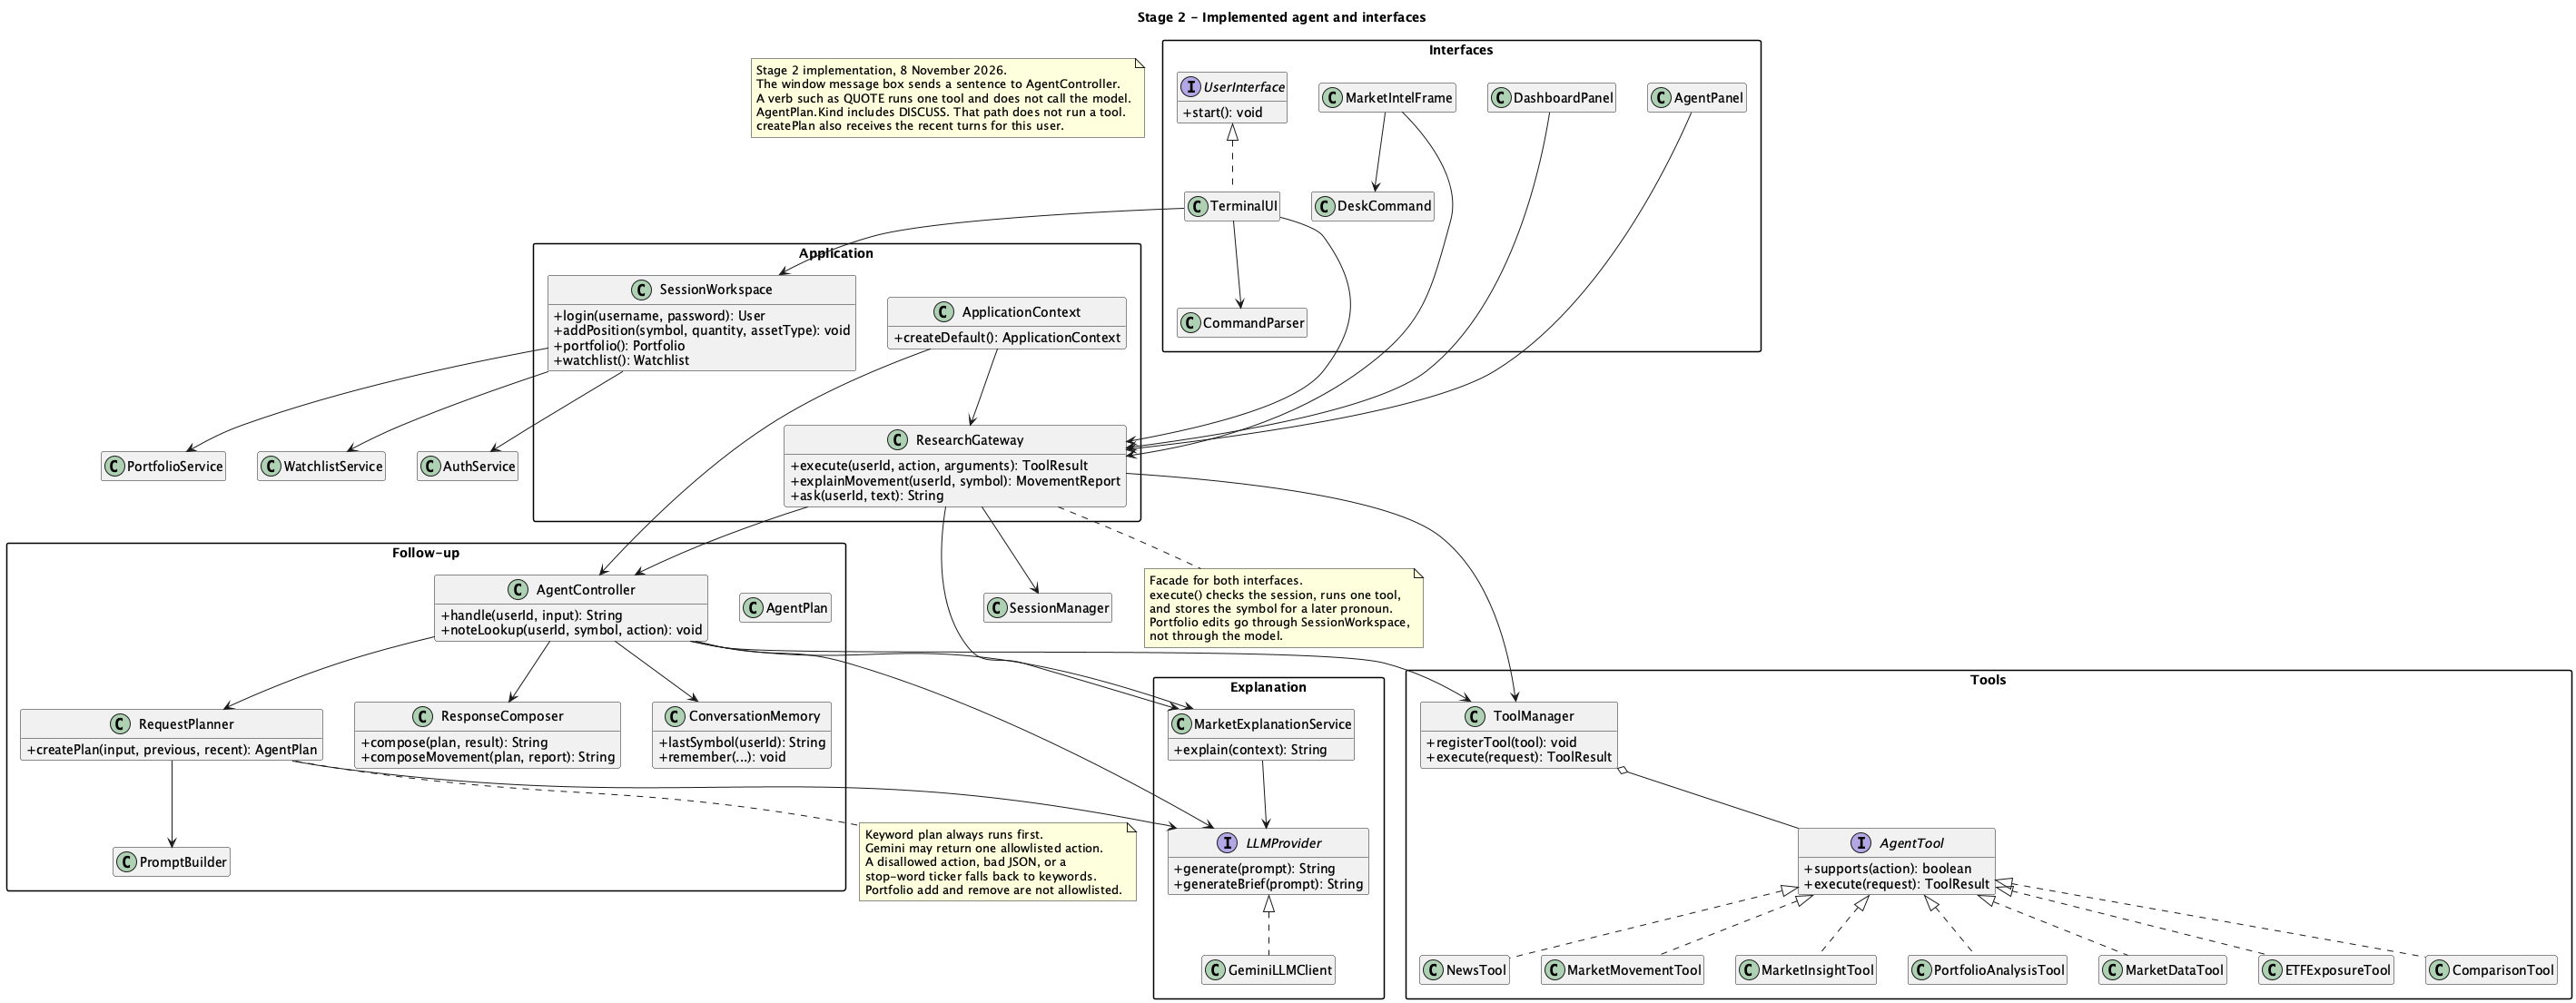
\includegraphics[width=\textwidth,height=0.72\textheight,keepaspectratio]{class-diagram-agent.png}
\caption{The window, the terminal, and the follow-up. A sentence goes through \texttt{AgentController}. A quote does not.}
\end{figure}

\begin{figure}[ht]
\centering
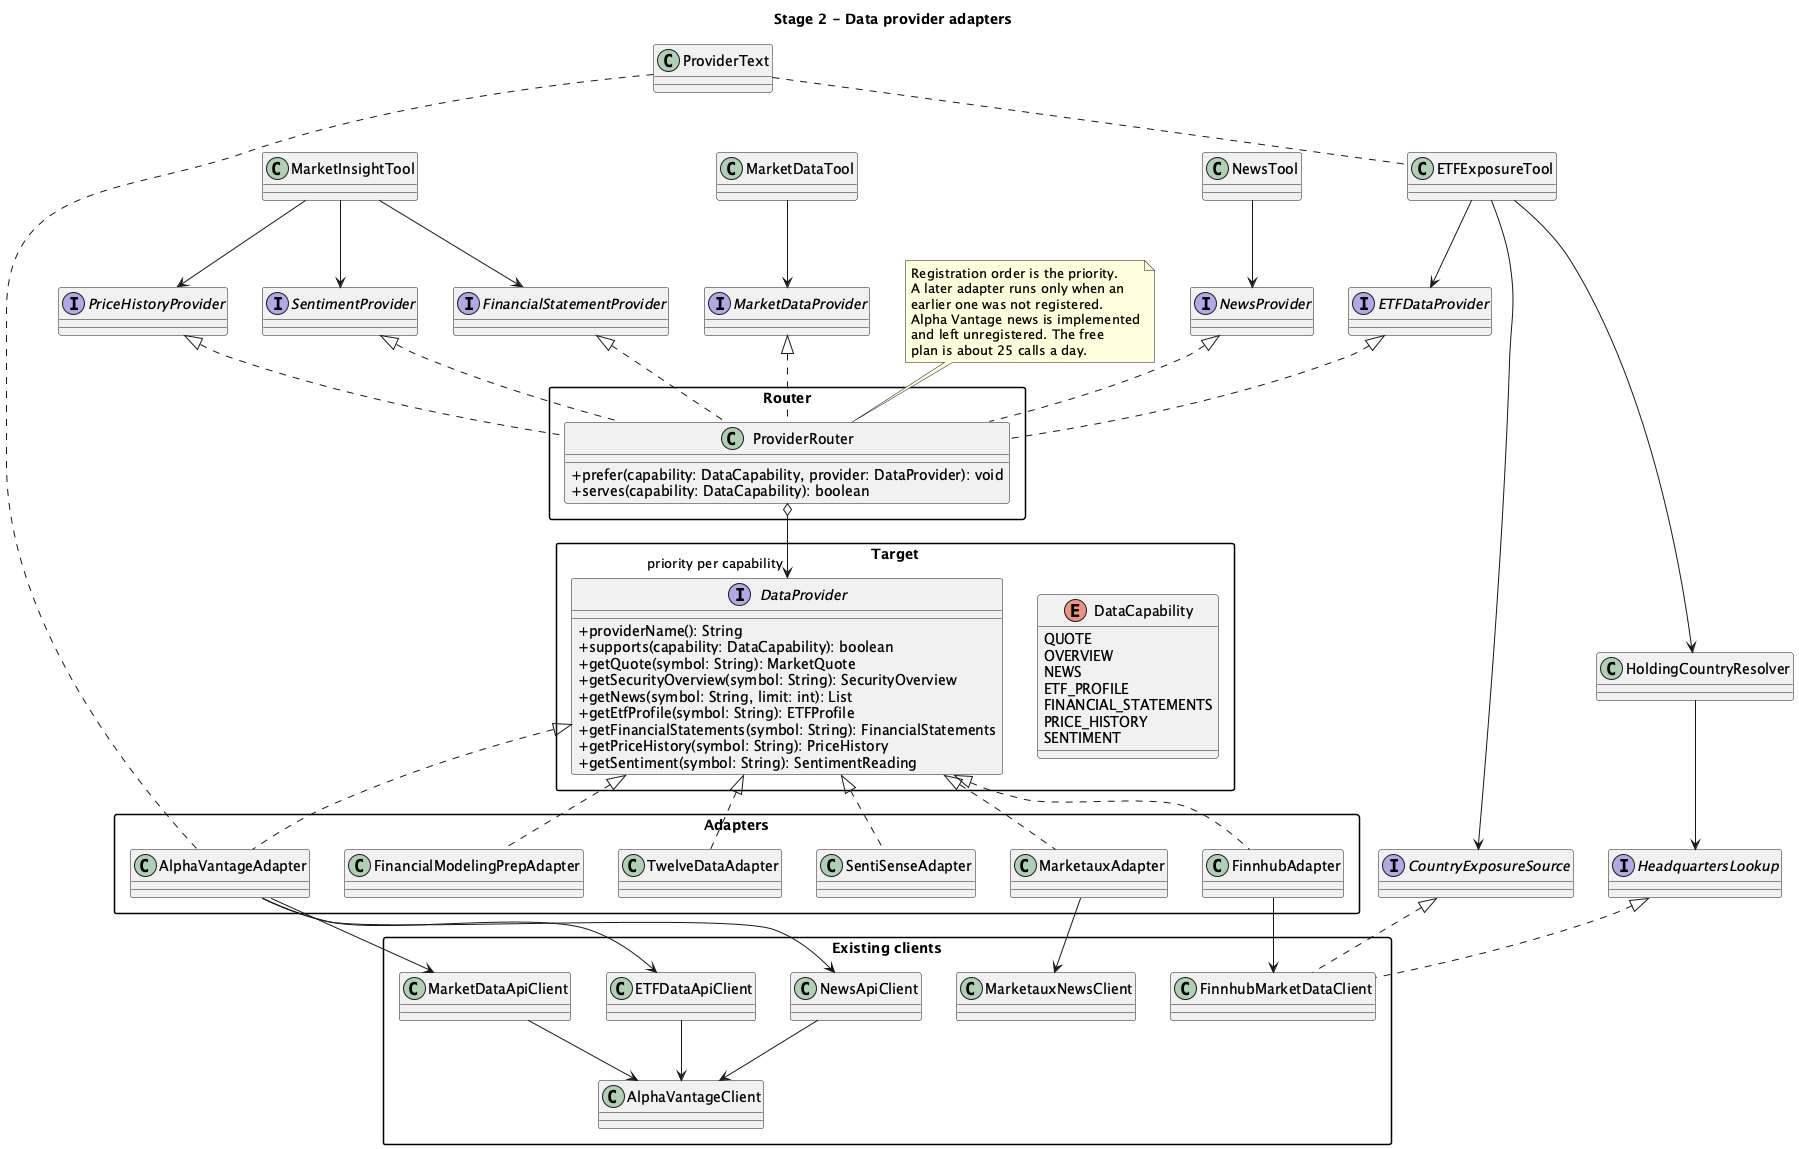
\includegraphics[width=\textwidth,height=0.72\textheight,keepaspectratio]{class-diagram-providers.png}
\caption{The adapters and \texttt{ProviderRouter}.}
\end{figure}

\begin{figure}[ht]
\centering
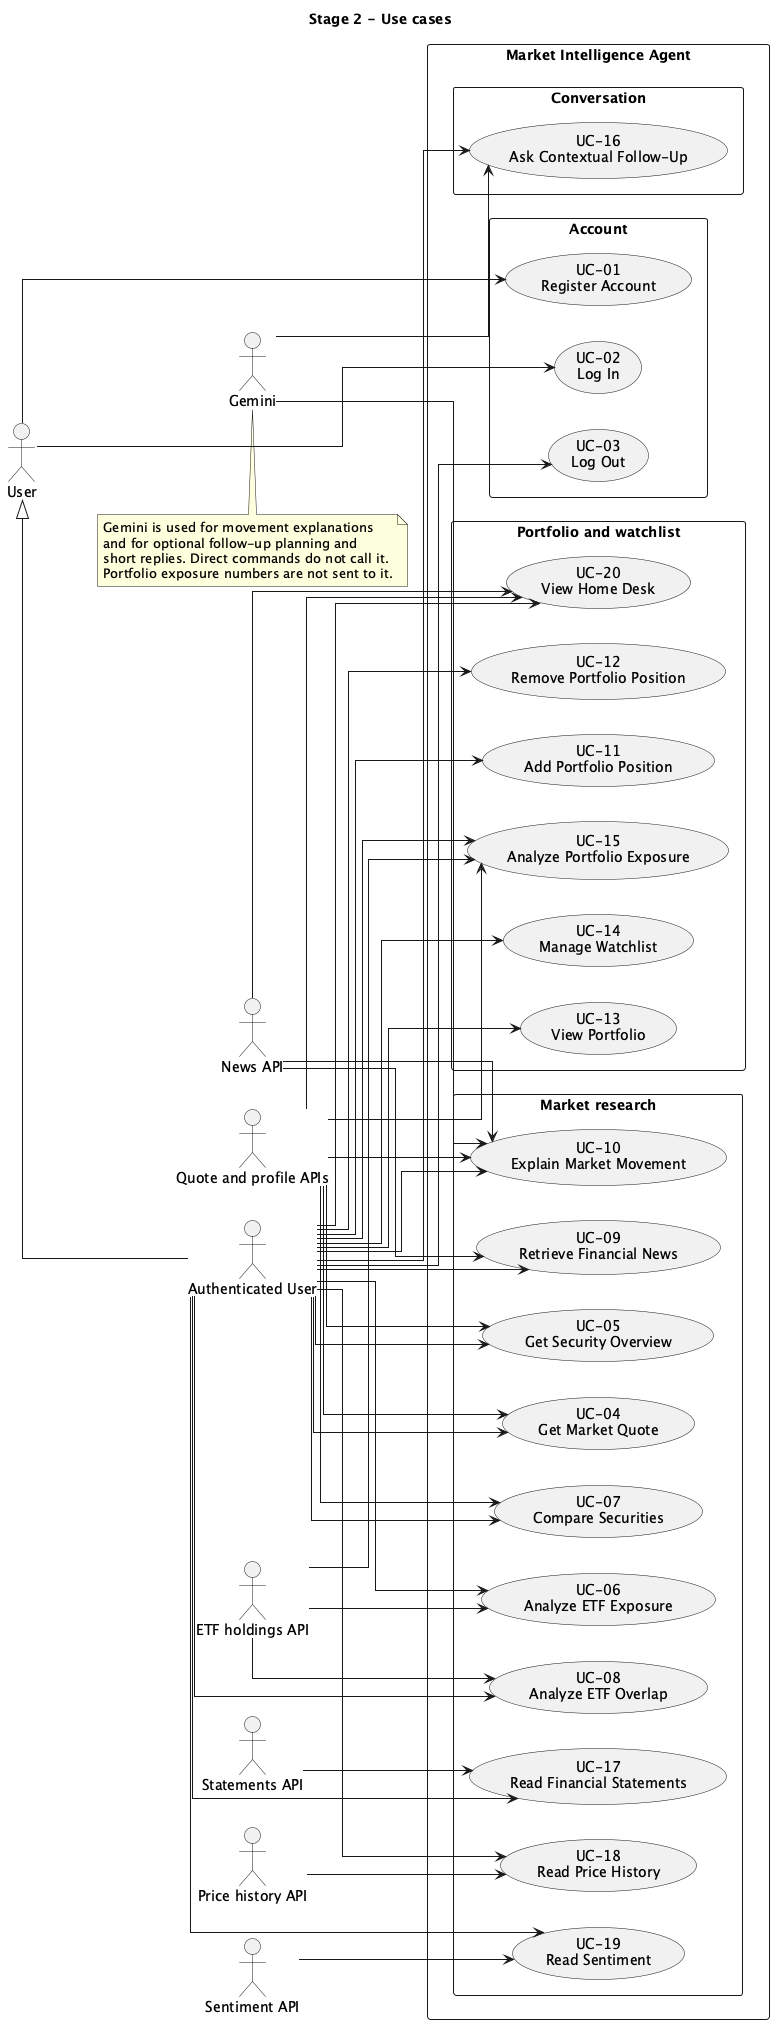
\includegraphics[width=\textwidth,height=0.55\textheight,keepaspectratio]{use-case-diagram.png}
\caption{Use cases. Gemini is only on the move note and the follow-up.}
\end{figure}

\begin{figure}[ht]
\centering
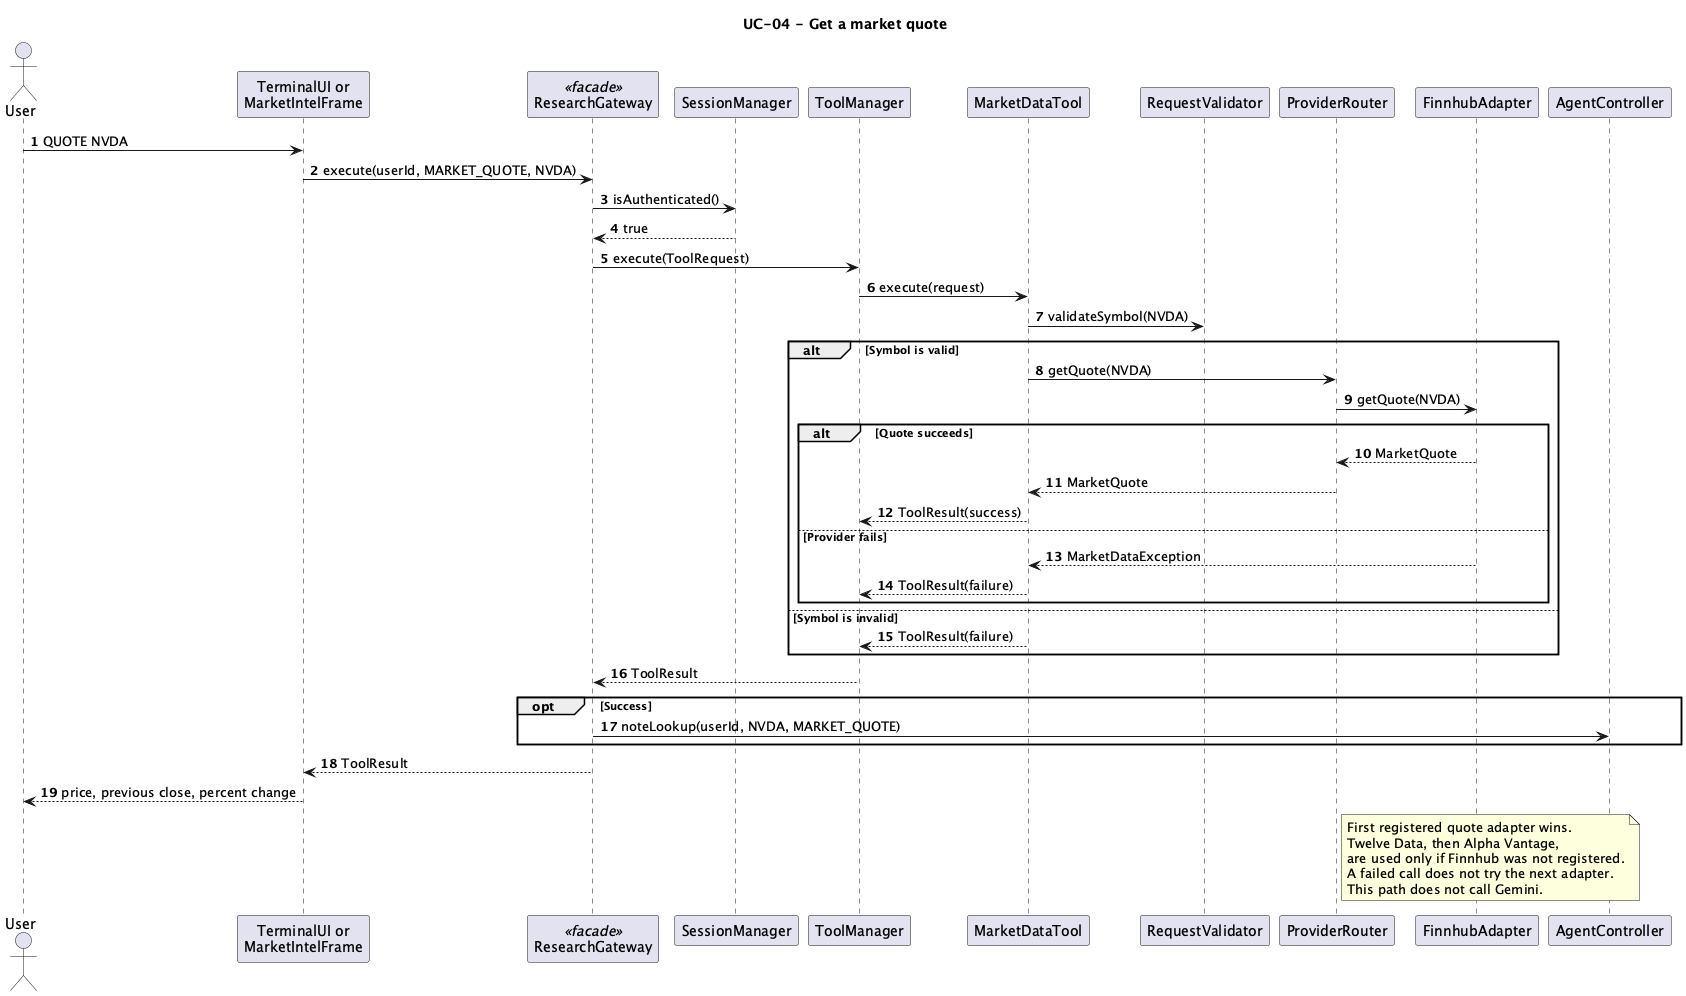
\includegraphics[width=\textwidth,height=0.42\textheight,keepaspectratio]{sequence-market-quote.png}
\caption{UC-04. A quote is a tool call.}
\end{figure}

\begin{figure}[ht]
\centering
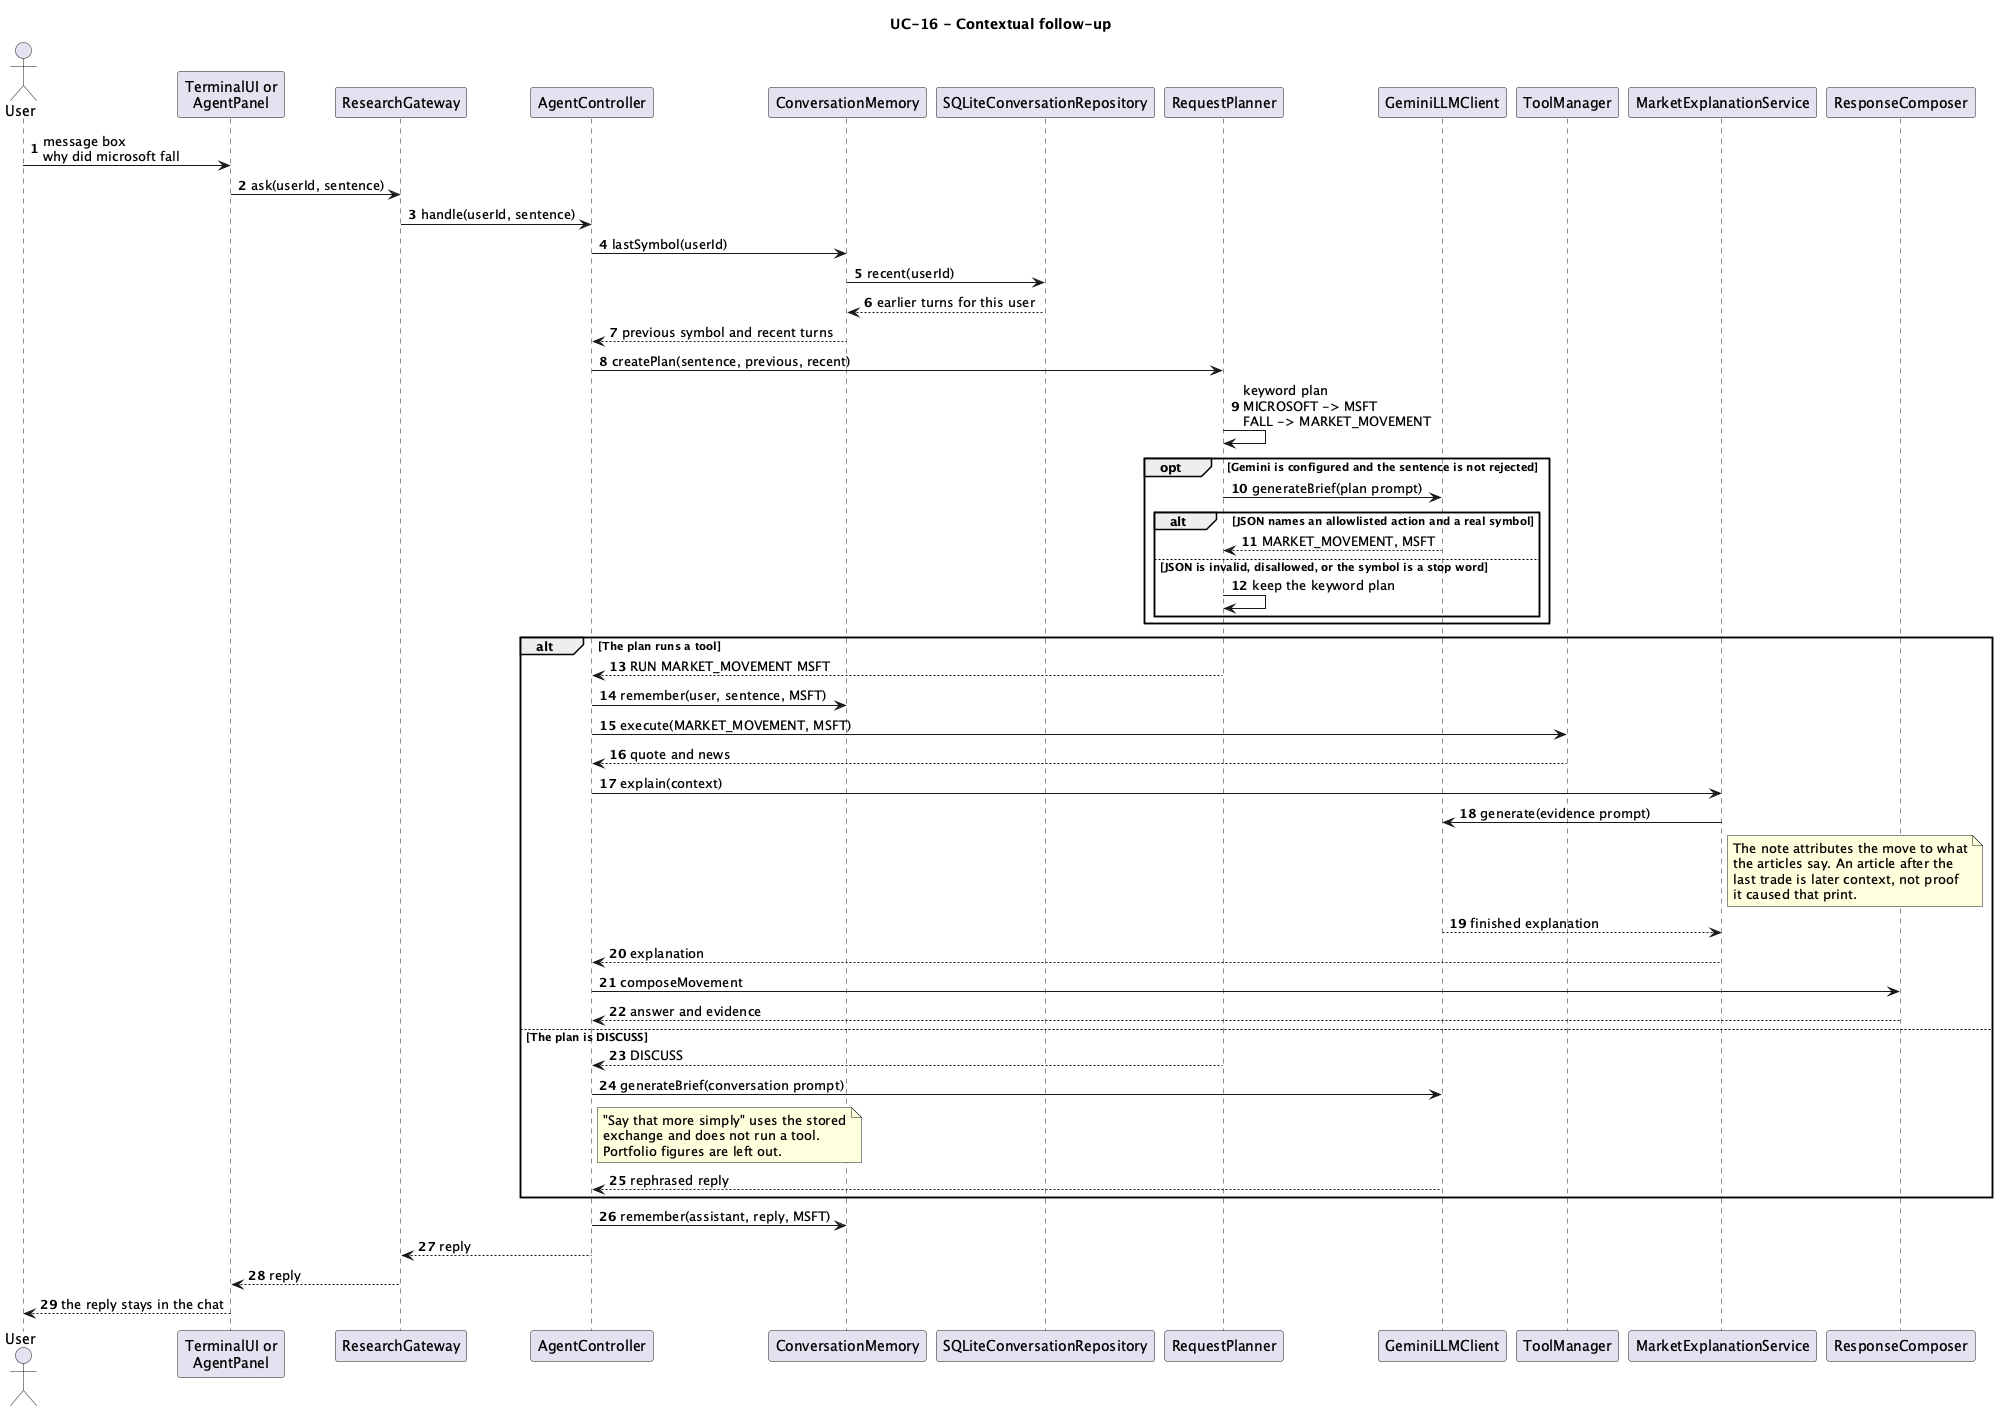
\includegraphics[width=\textwidth,height=0.62\textheight,keepaspectratio]{sequence-context-followup.png}
\caption{UC-16. A sentence is planned. A rephrase does not run a tool.}
\end{figure}

\begin{figure}[ht]
\centering
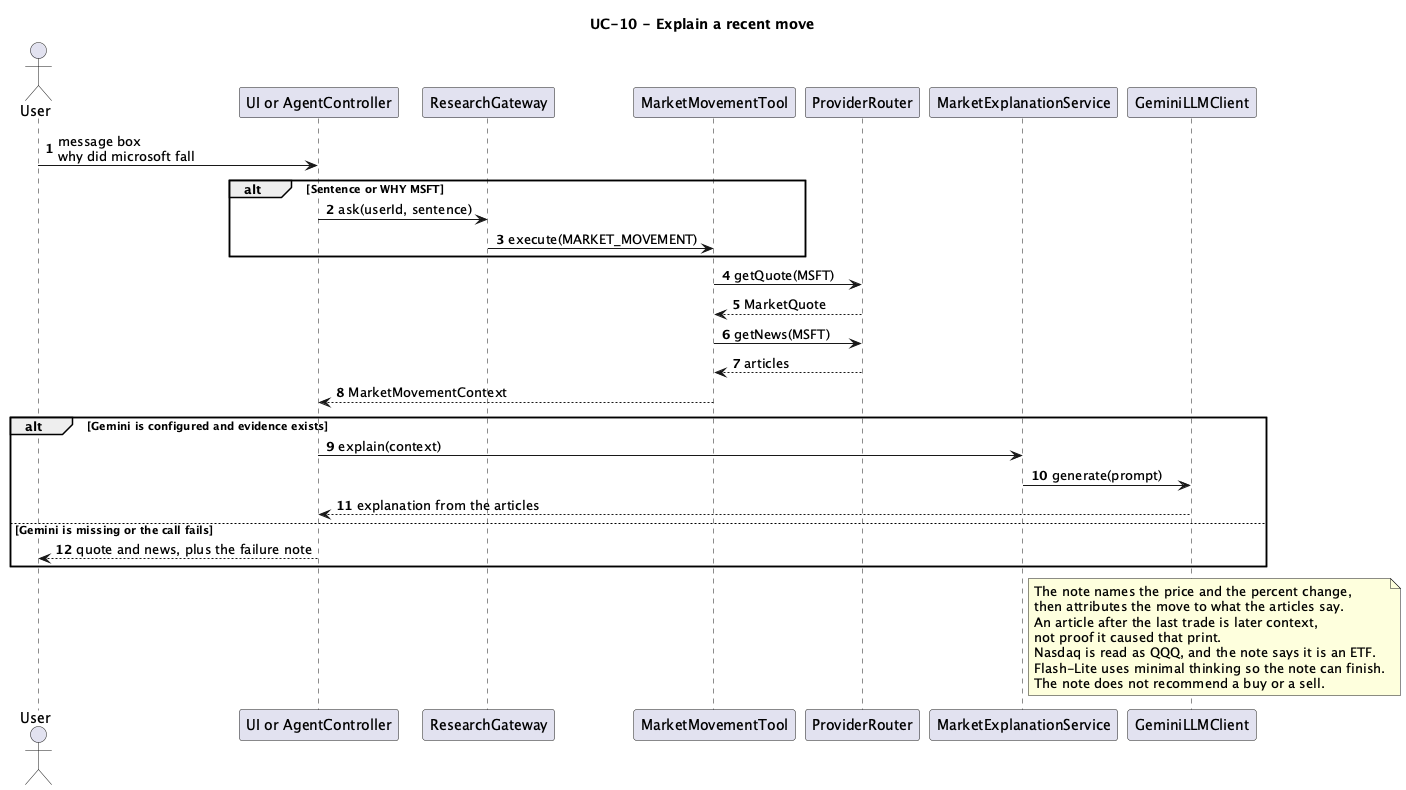
\includegraphics[width=\textwidth,height=0.48\textheight,keepaspectratio]{sequence-market-movement.png}
\caption{UC-10. Quote and news first. Gemini explains the move from the articles.}
\end{figure}

The other sources, for ETF analysis, country exposure, portfolio exposure, and the insight commands, are in \texttt{docs/stage2/uml/}. Rendered copies are in \texttt{docs/stage2/uml/rendered/}.

\section{Changes and rationale}

I kept the Stage~1 use cases. Where the running desk differs, this is why.

\textbf{Providers.}
Stage~1 had one client per provider interface, and Alpha Vantage was the market source.
I put six adapters behind \texttt{ProviderRouter}. Finnhub is first for quotes. Alpha Vantage is first for ETF holdings.
Alpha Vantage turned down a free educational plan, and the free tier is too small to carry the whole desk.
The tools still depend on the role interfaces. An unset key drops that adapter. UC-04, UC-05, and UC-09.

\textbf{Country exposure.}
Stage~1 was the fund's published country weights, then a model explanation.
I try Finnhub's country report. On HTTP 403 I map at most 25 holdings to headquarters countries, and I show the weights without calling Gemini.
The free plan returns 403. Filling in the rest would have been an invented allocation.
The user still gets a country breakdown, and the screen says it is headquarters, not the factsheet. UC-06.

\textbf{Where Gemini sits.}
Stage~1 sent every research use case through the model.
A verb such as \texttt{quote} runs one tool. Gemini is on the move note and on sentences.
A quote does not need a model, and a model there was inventing a sentence around a number I already had.
UC-04 through UC-09 and UC-15 stay deterministic. UC-10 and UC-16 are the hybrid ones.

\textbf{How a move is explained.}
Stage~1 had the composer ask the model to explain, including when evidence was missing.
I load the quote and the news first. The note has to use what the articles say, attribute the reason to the reporting, and still finish. An article after the last trade is later context, not proof.
The first notes were either cut off after the price, or they said the articles could not explain a move that the articles did discuss.
UC-10. \texttt{MarketExplanationService}, \texttt{generate}, minimal thinking on Flash-Lite.

\textbf{Portfolio exposure.}
Stage~1 had the model explain the exposure.
Java multiplies price by quantity. Those numbers are not sent to Gemini.
The figure is arithmetic. Narrating it invited a recommendation.
UC-15.

\textbf{Portfolio edits.}
Stage~1 put add and remove on the agent tools.
They stay on \texttt{SessionWorkspace}, off the allowlist.
A sentence must not change what I hold.
UC-11, UC-12, UC-14. There is no \texttt{PortfolioTool} class.

\textbf{The window.}
Stage~1 was a terminal.
I added the Swing desk, then replaced the command line with a message box so a sentence and a verb share one place.
Stage~2 asks for both a GUI and a CLI.
UC-20 is new. UC-16 is how the box talks to the planner.

\textbf{Non-interactive command line.}
The Stage~2 update asks for a program a terminal can run on a task file, for example \texttt{java -jar Agent.jar -LLMAPI -input task.txt}, because Stage~3 will call it that way.
I added a shaded jar, \texttt{target/Agent.jar}, and a batch path that reads \texttt{-input}, a pipe, or \texttt{-c}.
The interactive menu and the window are unchanged when those flags are absent and standard input is a terminal.
Batch mode cannot stop and ask for a password, so a missing account uses the local demo user \texttt{guest}.
\texttt{-LLMAPI} does not take a key. Keys stay in the environment.
Section~\ref{sec:batch-cli}.

\textbf{Statements, history, sentiment.}
These were not in the Stage~1 use-case set.
UC-17, UC-18, and UC-19, through \texttt{MarketInsightTool}.
The free adapters were already there for the provider pattern. The commands are the part a person can see.
Each one is unavailable when its key is unset. They do not replace a Stage~1 feature.

\textbf{Keys in errors.}
Stage~1 did not specify this. A live Alpha Vantage key showed up in a rate-limit message.
\texttt{ProviderText.redact} replaces that notice. I rotated the key. It is not in this report.

\section{AI tools and collaboration log}

Cursor is a \$20 a month subscription. Most of the work on this desk was with Grok 4.7 High Fast, and that model is included in the subscription. Over the past 30 days the Cursor account used 226.1 million tokens: 218.2 million of those were included, and 7.9 million were on-demand. The on-demand rows I pulled from the usage page come to \$1.86. Claude 4.5 Sonnet is \$1.59 of that, and Gemini 3.1 Pro is \$0.27. Those rows are about 3.0 million tokens, so they are not the whole 7.9 million. I am not filling in a dollar amount for the rows that are not on the page. Claude Fable was also used, inside the included allowance. The Gemini calls the running desk makes, through the API, are on the free tier.

\begin{center}
\small
\begin{tabularx}{\textwidth}{@{}p{2.7cm}Xp{2.6cm}@{}}
\toprule
Tool and model & What I used it for & Cost \\
\midrule
Cursor, mainly Grok 4.7 High Fast. Also Claude Fable, Claude 4.5 Sonnet, and Gemini 3.1 Pro. &
Most of the Java, the tests, the diagrams, and the drafts of this report. I ran the window myself and threw out the parts that were wrong. &
\$20 a month. Past 30 days: 226.1M tokens, 218.2M included and 7.9M on-demand. On-demand rows on the usage page total \$1.86. \\
\addlinespace
ChatGPT. The model name was not written down for the early design chats. &
The Stage~1 split into tools, providers, and repositories. &
Not written down. \\
\addlinespace
Gemini API, inside the running desk. Default \texttt{gemini-3.5-flash-lite}. I tried \texttt{gemini-3.8-flash} and \texttt{gemini-2.5-flash} and stopped using them. &
The move note, and the optional planning and replies on a sentence. Not quotes, not portfolio math, not add or remove. &
Free tier. No invoice. \\
\bottomrule
\end{tabularx}
\end{center}

The longer notes are in \texttt{docs/stage2/ai-collaboration-log.md}. The ones that actually changed the desk:

\begin{itemize}
\item Early on, ChatGPT proposed the tool and provider split. I added accounts, portfolios, SQLite, and \texttt{BigDecimal}. That split is still the package layout.
\item After Alpha Vantage declined a free educational plan, I asked for one adapter per vendor. That became \texttt{DataProvider} and \texttt{ProviderRouter}.
\item I saw HTTP 403 on country exposure, and then I saw my Alpha Vantage key in an error. The headquarters fallback and \texttt{ProviderText.redact} came out of that. I rotated the key.
\item Ordinary questions were missed, Gemini timed out, a new key got HTTP 404 from \texttt{gemini-2.5-flash}, and ``why did microsoft fall'' was read as the ticker DID. Memory, the allowlist, Flash-Lite, and the sentence parser came out of those runs. I checked the Microsoft question in the window.
\item The message box was still cutting the note off after the price, and a news reply was refusing to use the articles as the reason. The move note now has to finish, and it has to attribute the move to what the articles say.
\end{itemize}

The rule I kept, after the model was wired in, is that Gemini may interpret a question, but the numbers come from a tool. It does not get to edit the portfolio, and a sentence that tells it to ignore the instructions does not run anything.

\section{Development and verification summary}

Dates are Toronto dates on the public repository. I am not counting a merge commit as the work. The work is the commit that was merged. A report-only edit does not count as one of the five.

\subsection{Weekly commits}
Before 20 October the repository already had about twenty commits, from the Stage~1 design through the first terminal work. I work full time, so I did not push during the week of 20--26 October. New commits start again on 27 October.

Period~2, 27 October--2 November 2026, is over the minimum. Five of them:

\begin{itemize}
\item \href{https://github.com/xAssasinSoulx/market-intelligence-agent/commit/3770181a71225ac9e9eda009c9513fde0026fbe9}{3770181} -- 28 October. One wiring for the terminal and the window.
\item \href{https://github.com/xAssasinSoulx/market-intelligence-agent/commit/f1034052dedb7e04a8fbc2f5e3812880d99d6e91}{f103405} -- 28 October. The Swing window.
\item \href{https://github.com/xAssasinSoulx/market-intelligence-agent/commit/fcd3877976f4c873dd4e3c91e2056d3fbe8bb585}{fcd3877} -- 29 October. Exposure from price times quantity.
\item \href{https://github.com/xAssasinSoulx/market-intelligence-agent/commit/4da99b3b67d5395e7de4d11336206fa409d15825}{4da99b3} -- 29 October. Free APIs behind adapters.
\item \href{https://github.com/xAssasinSoulx/market-intelligence-agent/commit/c75e138a55b511dfe801579d0429c3fe0558c82c}{c75e138} -- 29 October. Follow-up from the last symbol.
\end{itemize}

Also that week: \texttt{6843eed} Finnhub quotes, \texttt{9716283} country exposure without printing keys, \texttt{1f4db1c} the home tape, \texttt{04de078} Gemini reading a question, \texttt{4f52ca0} Flash-Lite, and \texttt{931ec38} so ``why did microsoft fall'' stays a question.

Period~3, 3--9 November 2026, also clears five. I am not borrowing Period~2 commits for it.

\begin{itemize}
\item \href{https://github.com/xAssasinSoulx/market-intelligence-agent/commit/d5d220c}{d5d220c} -- 5 November. Home value, weight, and unpriced names.
\item \href{https://github.com/xAssasinSoulx/market-intelligence-agent/commit/1bcaa63}{1bcaa63} -- 6 November. One in-flight quote shared by the tape and the home book.
\item \href{https://github.com/xAssasinSoulx/market-intelligence-agent/commit/a0838f5}{a0838f5} -- 6 November. A real reason when a holding cannot be priced.
\item \href{https://github.com/xAssasinSoulx/market-intelligence-agent/commit/6eef95e}{6eef95e} -- 8 November. Terminal commands without a required slash.
\item \href{https://github.com/xAssasinSoulx/market-intelligence-agent/commit/f1d9eaf}{f1d9eaf} -- 8 November. The window box became a conversation.
\item \href{https://github.com/xAssasinSoulx/market-intelligence-agent/commit/9f71542}{9f71542} -- 8 November. The move note uses what the articles say.
\end{itemize}

\texttt{d7aa5d3} the same day lets a follow-up continue the last reply, and \texttt{1ae3345} stops a note from ending after the price.

\subsection{What I checked}
\texttt{./mvnw test} does not call the live APIs. \texttt{GeminiLiveSmokeTest} runs only if I set \texttt{RUN\_GEMINI\_LIVE\_TEST=1} and a Gemini key. On 8~November the planner tests, the explanation-prompt tests, and the Gemini client tests passed after the article-explanation change.

I also used the window with real keys. That is how I found the defects below. The test suite does not replace that, and that does not replace the suite.

\subsection{Defects I hit and fixed}
The country URL returned HTTP 302. It now calls \url{https://api.finnhub.io/api/v1/etf/country}. HTTP 403 on that report is the free plan, not a rejected key. Quotes still work.

An Alpha Vantage error included the live key. \texttt{ProviderText.redact} strips it. I rotated the key.

\texttt{why did microsoft fall} was read as the symbol DID. A full sentence stays a question. \texttt{WHY MSFT} is still the short command.

The move note stopped mid-word after the price, because Flash-Lite was spending the token budget on thinking. Explanations now use minimal thinking and the longer call. A reply cut off by the token limit is not shown as a finished note.

A news answer said the articles did not explain the day's move, even when they discussed the 40\% correction, demand, and guidance. A question about a price rising or falling stays a movement explanation, and the note has to use what the articles say.

\subsection{Still open}
The recording is public. Country exposure on this plan is headquarters, and that is the behavior, not a placeholder. The heavier testing and the KUMA checks are Stage~3, which is what the Stage~2 instructions say. The window shots are in Section~\ref{sec:shots}. The batch transcript is the offline run.

\section{Demonstration index}
\label{sec:demos}

One recording shows the window and the terminal together. I say the use-case id at the start of each segment. The link is \url{https://www.youtube.com/watch?v=J7uWTaclC8k}.

\begin{center}
\small
\begin{tabularx}{\textwidth}{@{}p{2.2cm}Xp{2.2cm}@{}}
\toprule
Feature & What is on screen & Timestamp \\
\midrule
Intro & What the desk is, window and terminal side by side. &
\href{https://youtu.be/J7uWTaclC8k?t=0}{00:00} \\
UC-01 Register & Create-account screen, password confirmed, back to sign-on. &
\href{https://youtu.be/J7uWTaclC8k?t=53}{00:53} \\
UC-02 Log in & Wrong password, then a real sign-on. &
\href{https://youtu.be/J7uWTaclC8k?t=133}{02:13} \\
UC-04 Quote & \texttt{quote NVDA} on both. Price, previous close, percent change. &
\href{https://youtu.be/J7uWTaclC8k?t=221}{03:41} \\
UC-05 Overview & \texttt{overview NVDA}. Name, exchange, currency, industry. &
\href{https://youtu.be/J7uWTaclC8k?t=293}{04:53} \\
UC-06 Exposure & \texttt{sector QQQ}, \texttt{geo QQQ}, \texttt{geo NVDA}. &
\href{https://youtu.be/J7uWTaclC8k?t=364}{06:04} \\
UC-07 Compare & \texttt{compare NVDA MSFT}. &
\href{https://youtu.be/J7uWTaclC8k?t=539}{08:59} \\
UC-08 Overlap & \texttt{overlap QQQ SPY}. &
\href{https://youtu.be/J7uWTaclC8k?t=606}{10:06} \\
UC-09 News & \texttt{news NVDA}. A match is not, by itself, the cause. &
\href{https://youtu.be/J7uWTaclC8k?t=698}{11:38} \\
UC-10 Move & \texttt{why did microsoft fall} and \texttt{why is intel up}. &
\href{https://youtu.be/J7uWTaclC8k?t=760}{12:40} \\
UC-16 Follow-up & Sector of the last symbol, a simpler wording, then a rejected instruction. &
\href{https://youtu.be/J7uWTaclC8k?t=952}{15:52} \\
UC-11 Add & \texttt{port add NVDA 10 STOCK}. &
\href{https://youtu.be/J7uWTaclC8k?t=1133}{18:53} \\
UC-13 View & The stored portfolio on both screens. &
\href{https://youtu.be/J7uWTaclC8k?t=1243}{20:43} \\
UC-20 Home & Value, day move, the position row, and the tape. &
\href{https://youtu.be/J7uWTaclC8k?t=1298}{21:38} \\
UC-15 Exposure & \texttt{exposure}. Price times quantity. &
\href{https://youtu.be/J7uWTaclC8k?t=1364}{22:44} \\
UC-14 Watchlist & Add AAPL, then remove it. &
\href{https://youtu.be/J7uWTaclC8k?t=1473}{24:33} \\
UC-12 Remove & Remove NVDA, then a symbol that is not held. &
\href{https://youtu.be/J7uWTaclC8k?t=1564}{26:04} \\
UC-17 Statements & \texttt{statements NVDA}. &
\href{https://youtu.be/J7uWTaclC8k?t=1631}{27:11} \\
UC-18 History & \texttt{history NVDA}. Bars and RSI. &
\href{https://youtu.be/J7uWTaclC8k?t=1692}{28:12} \\
UC-19 Sentiment & \texttt{sentiment NVDA}. Score and band. &
\href{https://youtu.be/J7uWTaclC8k?t=1759}{29:19} \\
UC-03 Log out & Window back to sign-on. Terminal back to the menu. &
\href{https://youtu.be/J7uWTaclC8k?t=1815}{30:15} \\
Close & Both interfaces, same features. &
\href{https://youtu.be/J7uWTaclC8k?t=1876}{31:16} \\
\bottomrule
\end{tabularx}
\end{center}

\end{document}
